%!TEX root = main.tex
\section{Towards Dataset Understanding\label{sec:understanding}}
\subsection{Challenges}
\begin{itemize}
\item Problem of cold-start recommendation (as discussed earlier use may not always know what to query for)
\item related works have focussed on making specification easier , but not really trying to understnad user intent or what might the user want to see.
\item Within a dataset, structure and provenance is essential to help users navigate and provide users with sense of coverage and completion. This is an important but underexplored area. (viz-sum, Sarvghad et al 2017)
\item provenance of schema and attribute understanding (coverage, etc) 
\end{itemize}
Recommendation providing better understanding for overall dataset
For example, in \zv 
%providing overview recommendations (representative trends and outliers)

\subsection{\sbd: Navigating Through Data Slices with Hierarchical Summary of Visualizations}
%understanding distributions (distribution awareness)
%introduce problem + challenge
\par Common analytics tasks, such as causal inference, feature selection, and outlier detection requires studying the distributions or patterns at different levels of data granularity~\cite{Anand2015,Wu2013,Heer2012}. However, without knowing \textit{what} subset of data contains an insightful distribution, manually exploring distributions from all possible data subsets can be tedious and inefficient. first, constructing the large number of visualizations corresponding to all possible data subsets, and then, navigating through this large space of visualizations to draw meaningful insights is challenging, particularly because there is no systematic way to perform these exercises.

% explain what storyboard does
\par To this end, we present \system, an interactive visualization summarization system that automatically selects a small set of visualizations to summarize the distributions within a dataset in an informative manner. Nevertheless, finding effective visualizations to summarize a dataset is not as trivial as picking individual visualizations that maximizes some statistical measure, such as deviation~\cite{Vartak2015}, coverage~\cite{Sarvghad2017}, or significance testing~\cite{Anand2015}, which can often result in misleading summarizations. The above example demonstrates a scenario where the selection of an improper reference (female) for comparing the visualization (black female) against results in misleading insights. In \system, we formulate an objective where a visualization is \emph{actually} interesting when it deviates from and can not be explained by \emph{even} its most informative reference.
% one paragraph on motivation on objectives and explain lattice + traversal 
\begin{figure}[h!]
\label{fig:modalities}
\centering
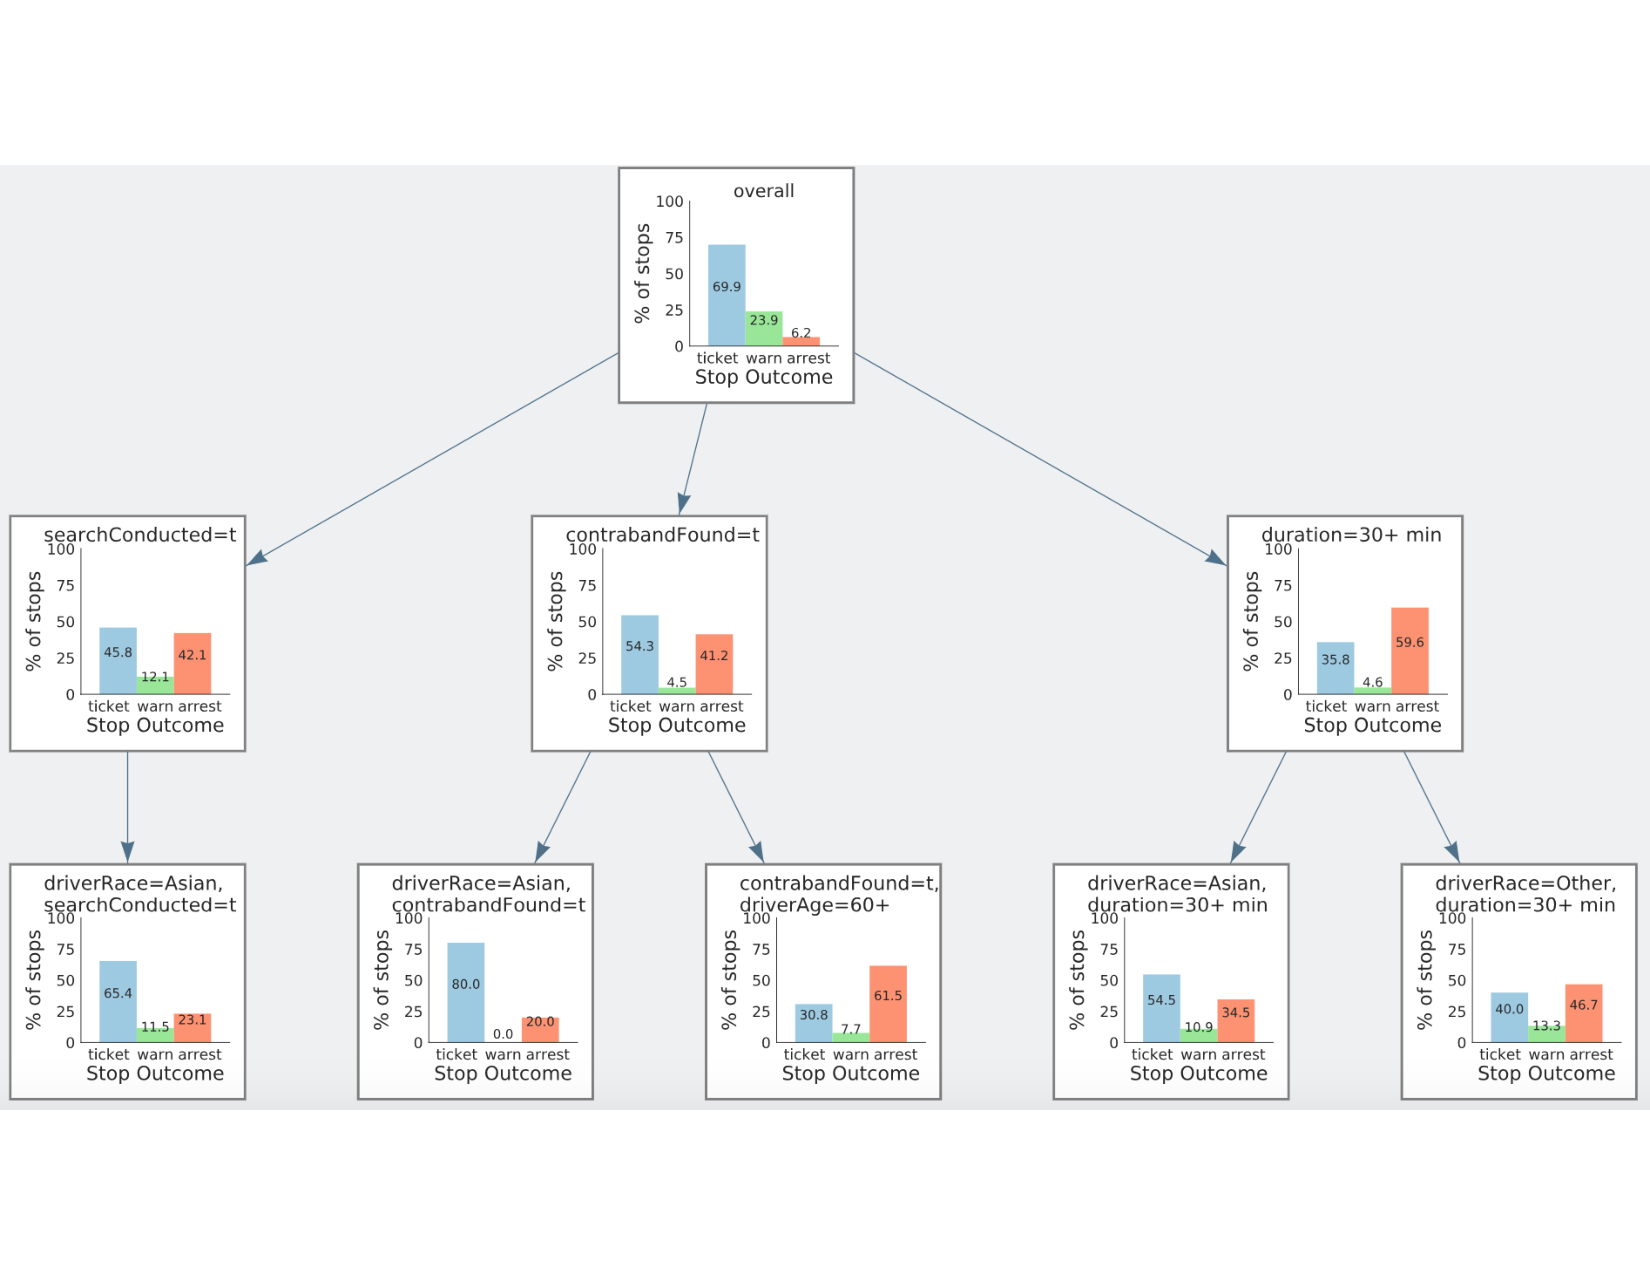
\includegraphics[width=0.7\linewidth]{figures/storyboard.pdf}
\caption{Example dashboard with generated from the Police Stop Dataset \cite{police}, which contains records of police stops that resulted in a warning, ticket, or an arrest. The attributes in the dataset include driver gender, age, race, and the stop time of day, whether a search was conducted, and whether contraband was found. We generate a dashboard of visualizations with bar charts with x-axis as the stop outcome (whether the police stop resulted in a ticket, warning, or arrest/summons) and y-axis as the percentage of police stops that led to this outcome.}
\end{figure} 
User study show that user is able to make better predictions regarding unseen visualizations, determine attribute influence, and ------, compared to baselines.
%explain distribution awareness + its application, its relationship with dataset understnading + how it can be used in other contexts.
\par Our system is motivated by our observation that when an analyst is aware of the distributions present in different data subsets, she can draw meaningful insights and establish correlations about related visualizations that she has not yet seen with ease. We define this aspect of dataset understanding as \emph{distribution awareness}. 



Data is agnostic to the user, intention ---, by building tools---, Section \ref{sec:precise} to \ref{sec:vague} have focussed on extracting what user want from data. bridging together what user want from data, what data has to offer, supporting interactive discourse between the two. 
 Either using one-size-fits-all statistics, templates, heuristics as a solution or problem only applicable to a subset of analytic tasks\cite{Vartak2015,Vartak2017}. 
